\documentclass[11pt,a4paper]{article}
\usepackage[T1]{fontenc}
\usepackage[utf8]{inputenc}
\usepackage{lmodern}
\usepackage[margin=23mm]{geometry}
\usepackage{amsmath,amssymb,booktabs,longtable,array,graphicx,xcolor,microtype}
\usepackage{xurl}
\usepackage[colorlinks=true,linkcolor=blue!45!black,citecolor=blue!45!black,urlcolor=blue!45!black,breaklinks=true]{hyperref}
\emergencystretch=2em
\setlength{\parskip}{4pt}
\setlength{\parindent}{0pt}
\newcommand{\doctype}{Technical report}
\newcommand{\docversion}{v0.01.001}
\newcommand{\docdate}{1 November 2026}
\newcommand{\versiondoi}{10.5281/zenodo.23851639}
\newcommand{\conceptdoi}{10.5281/zenodo.23851364}
\newcommand{\docrepo}{github.com/fsantibanezleal/CAOS\_OreBridge}
\newcommand{\headerblock}{\begin{center}\fbox{\parbox{0.94\textwidth}{\small\raggedright
\textbf{\doctype}\quad$\cdot$\quad\docversion, \docdate\quad$\cdot$\quad Licence CC BY 4.0\\[2pt]
CAOS open-research programme\quad$\cdot$\quad OreBridge\\[2pt]
Version DOI: \href{https://doi.org/\versiondoi}{\texttt{\versiondoi}}\\
Concept DOI (always latest): \href{https://doi.org/\conceptdoi}{\texttt{\conceptdoi}}\\[2pt]
Not peer reviewed. Source code, data and computational results:\\
\href{https://github.com/fsantibanezleal/CAOS_OreBridge}{\texttt{\docrepo}}
}}\end{center}\vspace{4pt}}
\title{Connected plant visualization with timestamped observations and versioned process-engine evidence}
\author{Felipe Santibáñez-Leal\\\small CAOS open-research programme, Santiago, Chile\\\small ORCID: 0000-0002-0150-3246}
\date{}
\begin{document}
\maketitle
\headerblock
\begin{abstract}
Plant observations are difficult to interpret when equipment identity, engineering units, process relationships and time support are fragmented across views. OreBridge connects an authored copper-processing complex of 36 assets and 47 streams to synchronized three-dimensional geometry, diagrams, trends and source evidence. Four released Python engines are executed and ten public CAOS artifacts verified at immutable source identifiers. An optional authenticated read-only OPC UA adapter preserves source-change, server-confirmation and arrival times. A controlled sixteen-channel network compares thresholds, constrained reconciliation, a fitted causal histogram predictor and transport-aware fusion over 6144 method/scenario cells. TASC recall is 0.3419, compared with 0.8399 for the predictor and 0.5191 without topology. An additional regularized linear causal model is fitted separately and evaluated on the same already-known test slots: 768 new ridge evaluations accompany 768 reused histogram rows. Ridge recall is 0.9204, with false-positive rate 0.02921 versus 0.01591 for the histogram predictor. Seed-block intervals preserve dependence; the extension is not prospectively untouched validation. Independent constrained and linear-algebra checks, source recomputation, timestamp tests and a settling-grid study distinguish numerical consistency from applicability. The evidence supports working integration and reproducible controlled models, without establishing field detection, automatic diagnosis or facility safety.
\end{abstract}
\clearpage
\tableofcontents
\clearpage

\section{Problem and scope}
A plant engineer may inspect a flow reading, a motor-condition example, a mass-balance residual and a vessel model in different tools. Those quantities do not describe the same physical state merely because they share an equipment name. A reading needs an unambiguous asset, a quantity and unit, an observation time, source quality and a defined relationship to the displayed process. A model adds assumptions and uncertainty rather than turning itself into an instrument.

The central object here is one connected visual plant. Selecting equipment in geometry, a directed diagram or a keyboard control selects the same graph asset and its upstream/downstream context. Time-series and scalar displays retain the evidence time of their numerical interpretation. Existing CAOS calculations enter through their released interfaces or public result artifacts, instead of private-module copying or independent calculator panels.

The authored layout represents distinct sulfide-concentrator and oxide-leach routes, with shared ore arrival and water context. It has 36 assets and 47 directed streams. Its dimensions establish a coherent reference coordinate system; they are not an as-built survey. Sixteen instrument-like channels support a controlled transport experiment. Other equipment has geometry and reference context without invented sensor histories. No operating historian, production credentials, site geometry or operator acceptance was available.

Energy and water provide relevant industrial context, but a visualization does not itself demonstrate savings. Chilean copper-sector projections describe increasing electricity use and growing seawater reliance~\cite{cochilco-energy,cochilco-water}. These sector observations motivate joined process context. Economic value, improved decisions or reduced resource consumption would require an independent operating-site study.

\section{Related systems and modeling choices}
\subsection{Geometry and semantic identity}
Azure 3D Scenes and AWS IoT TwinMaker already connect spatial elements, entities, data-driven behavior and graph relationships~\cite{azure,aws}. Three-dimensional data binding is therefore an established capability. The question examined here is whether a small independently reproducible implementation preserves identity, time support and provenance across its own views. No platform-superiority claim follows from reproducing a visual pattern.

Khronos glTF provides hierarchical nodes, transforms and application extras~\cite{gltf}. OreBridge uses a unique \texttt{extras.assetId} to bind an imported node to graph equipment. DEXPI addresses structured plant/process engineering exchange~\cite{dexpi}; the bounded asset graph is not a complete DEXPI implementation. Likewise, mining information definitions provide a semantic reference without establishing conformance to the full OPC UA Mining companion specification~\cite{mining}.

\subsection{Observation time and reconciliation}
An OPC UA DataValue distinguishes status, source time and server time~\cite{datavalue}. Source time may denote the last value or status change, while server time can confirm an unchanged value. Treating every old source-change timestamp as stale would reject healthy constant signals. The adapter therefore requires a stated policy and retains both timestamps, rather than collapsing them into a browser arrival time.

Constrained reconciliation is established in mineral processing~\cite{sadeghi}. Conservation reduces inconsistent measurement combinations to a feasible state, subject to uncertainty assumptions and observability. Huber loss limits the influence of large standardized innovations~\cite{huber}. Neither conservation closure nor robust optimization proves the cause of a process discrepancy. This distinction is central when an equipment color accompanies a mathematical residual.

\subsection{Learned temporal comparisons}
Graph-based multivariate forecasting and detection have prior literature, including GDN~\cite{gdn}; missing observations also motivate dedicated spatiotemporal methods~\cite{gstpro}. Those methods are cited as related work and are not executed comparators here. The actual trained comparison uses maintained histogram gradient boosting~\cite{hgb}, with a separate regressor for every channel and four causal multichannel lags. Its inclusion establishes a reproducible learned comparison, without implying global best performance.

\section{Plant graph and physical quantities}
\subsection{Equipment, streams and coordinate system}
The plant includes extraction/loading context, run-of-mine stockpile, primary and secondary crushing, feed bin, grinding/classification, rougher/cleaner flotation, concentrate thickening/filtering, tailings thickening, recovered/make-up water, leach, solvent extraction, electrowinning and utility context. Equipment geometry is distinct by type. Mill charge, stockpile terrain and other external engine examples remain separate evidence, rather than being interpreted as the geometry generator for every displayed mesh.

Coordinates use metres with vertical $Y$. Directed stream identity is independent of geometry. A stream carries material, nominal rate, unit, delay and separately represented water volume where applicable. Dry solids in tonnes per hour cannot be added to slurry volume or electrical power. The nominal concentrator routes 720\,t/h fresh dry solids and 1800\,t/h recycle through a 2520\,t/h combined grinding reference. The combined circuit channel must not be mistaken for the fresh feed of one SAG vessel.

\begin{figure}[htbp]\centering
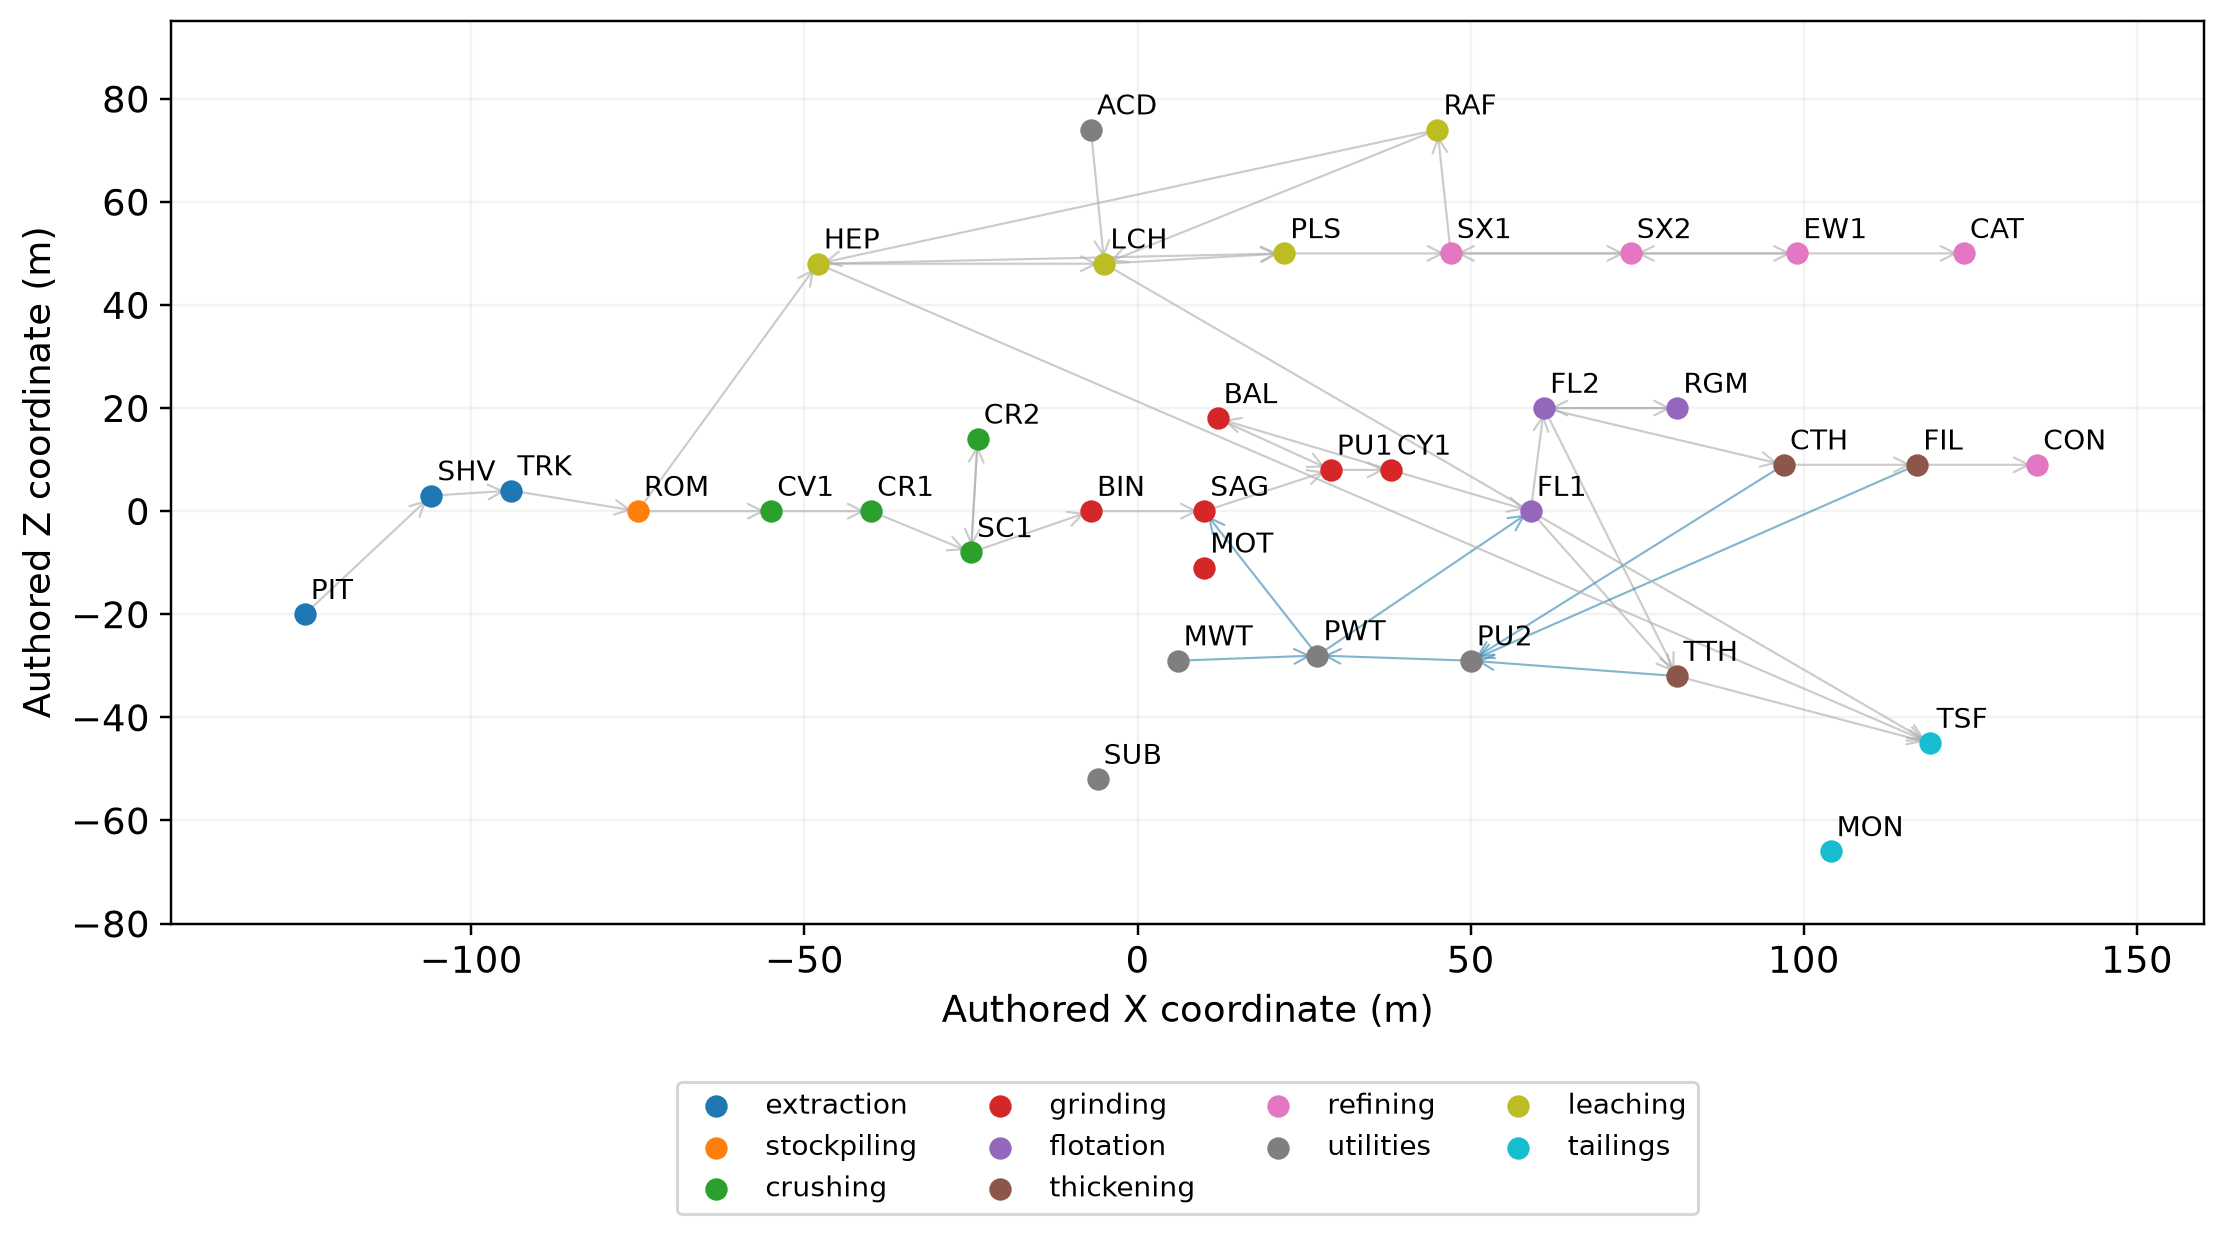
\includegraphics[width=\textwidth]{../shared/plant-map.png}
\caption{Authored reference layout in horizontal coordinates. Arrows preserve graph direction; water is distinguished from other material context. This is a synthetic engineering layout, not a surveyed facility.}
\end{figure}

\subsection{Accounting and separate model bases}
The nominal water accounting supplies 415\,m$^3$/h, divided into 265\,m$^3$/h recovered water and 150\,m$^3$/h make-up. The authored water delivered to grinding and flotation is tracked separately from dry solids. A closed accounting graph does not imply that every nominal hydrodynamic state is feasible. The finite-volume settling reference uses its own flow and geometry, rather than calibrating the displayed plant thickener.

The concentrate and cathode products are separate boundaries. The ideal leach/SX/EW example uses a 100\,t/h feed at copper fraction 0.005. A different oxide route does not establish that all ores can be routed interchangeably through flotation or chemical extraction. No mineral-general kinetic law or industrial operating prescription is inferred from those reference inputs.

\section{Observation contract and read-only access}
\subsection{Identity, units and accepted state}
The graph includes a semantic catalog fixing tag identifier, asset identifier and canonical unit. The gateway configuration must match that tuple. A source unit may differ only within a supported dimension. For example, 100\,kg/s becomes 360\,t/h. Conversion overflow, non-finite values, an unsupported dimension or an out-of-domain quantity cannot become a zero-valued healthy reading.

Each observation preserves value or explicit absence, quality, source time, server time, arrival time, delivery sequence and freshness basis. The default maximum freshness window is 15\,s, with 2\,s future-clock tolerance. Time strings require an explicit timezone. Accepted delivery sequences increase and source times cannot regress. The browser independently checks the graph revision and binding before replacing its accepted connection state.

\subsection{Freshness and its limits}
With source-based freshness, the observation must have a recently renewed source timestamp. With server-based freshness, a current server confirmation may retain a constant value whose source-change time is older. Both remain available for interpretation. Fresh server confirmation proves availability from that server under the configured policy; it does not prove that a physical sensing element cannot freeze. That distinction needs source-specific heartbeat or diagnostic information.

The local adapter makes one allow-listed batch read, preserving individual DataValue status. A missing node is unavailable without erasing the valid state of another configured node. The browser keeps a bounded connection history and leaves gaps for rejected sources. Carry-forward preparation inside a forecast feature vector is never displayed as a new observed value.

\subsection{Transport and authorization boundary}
Remote OPC access requires signed encrypted transport and a server certificate. The web boundary requires a bearer token and explicit origins; the token stays in browser memory and clears on disconnect. Unencrypted OPC is restricted to an explicitly enabled loopback test. Security mechanisms and trust remain application responsibilities~\cite{opc-security}.

The implemented surface is read-only: there is no write, setpoint, PLC method, dispatch or control endpoint. Public static delivery contains no site endpoint, node identifiers or private certificates. Connecting a new source requires its own mapping and source policy. The synthetic replay's trained detectors do not silently begin scoring new site instruments.

\section{Spatial synchronization and interaction}
\subsection{A common snapshot}
The workbench shares selected asset, case, method, snapshot availability time, source and graph traversal across geometry, diagram, scalar values and trends. The graph defines equipment identity; a label or mesh name alone is insufficient. Engine references form a separate information layer, with their original case descriptions and units. Equipment without an observation channel remains context instead of receiving a fabricated time series.

For aligned method $m$, the exported evidence lag $\ell_{m,j}$ identifies the raw reading used for channel $j$:
\begin{equation}
 t_{e,m,j}=t_a-\ell_{m,j},\qquad
 \ell_{m,j}=D-d_j\quad\hbox{for parcel-aligned methods},
 \label{eq:evidence}
\end{equation}
where $D=14$\,s is the largest authored delay, $d_j$ is channel delay and $t_a$ is snapshot availability. Unaligned methods use zero lag. Scalar value, validity and color resolve the same evidence reading as the score. A trend comparing TASC state with observations uses aligned observations and truth on the availability axis. This prevents a causally older alarm from being attached to a newer raw value merely because both occupy array row $t_a$.

\begin{figure}[htbp]\centering
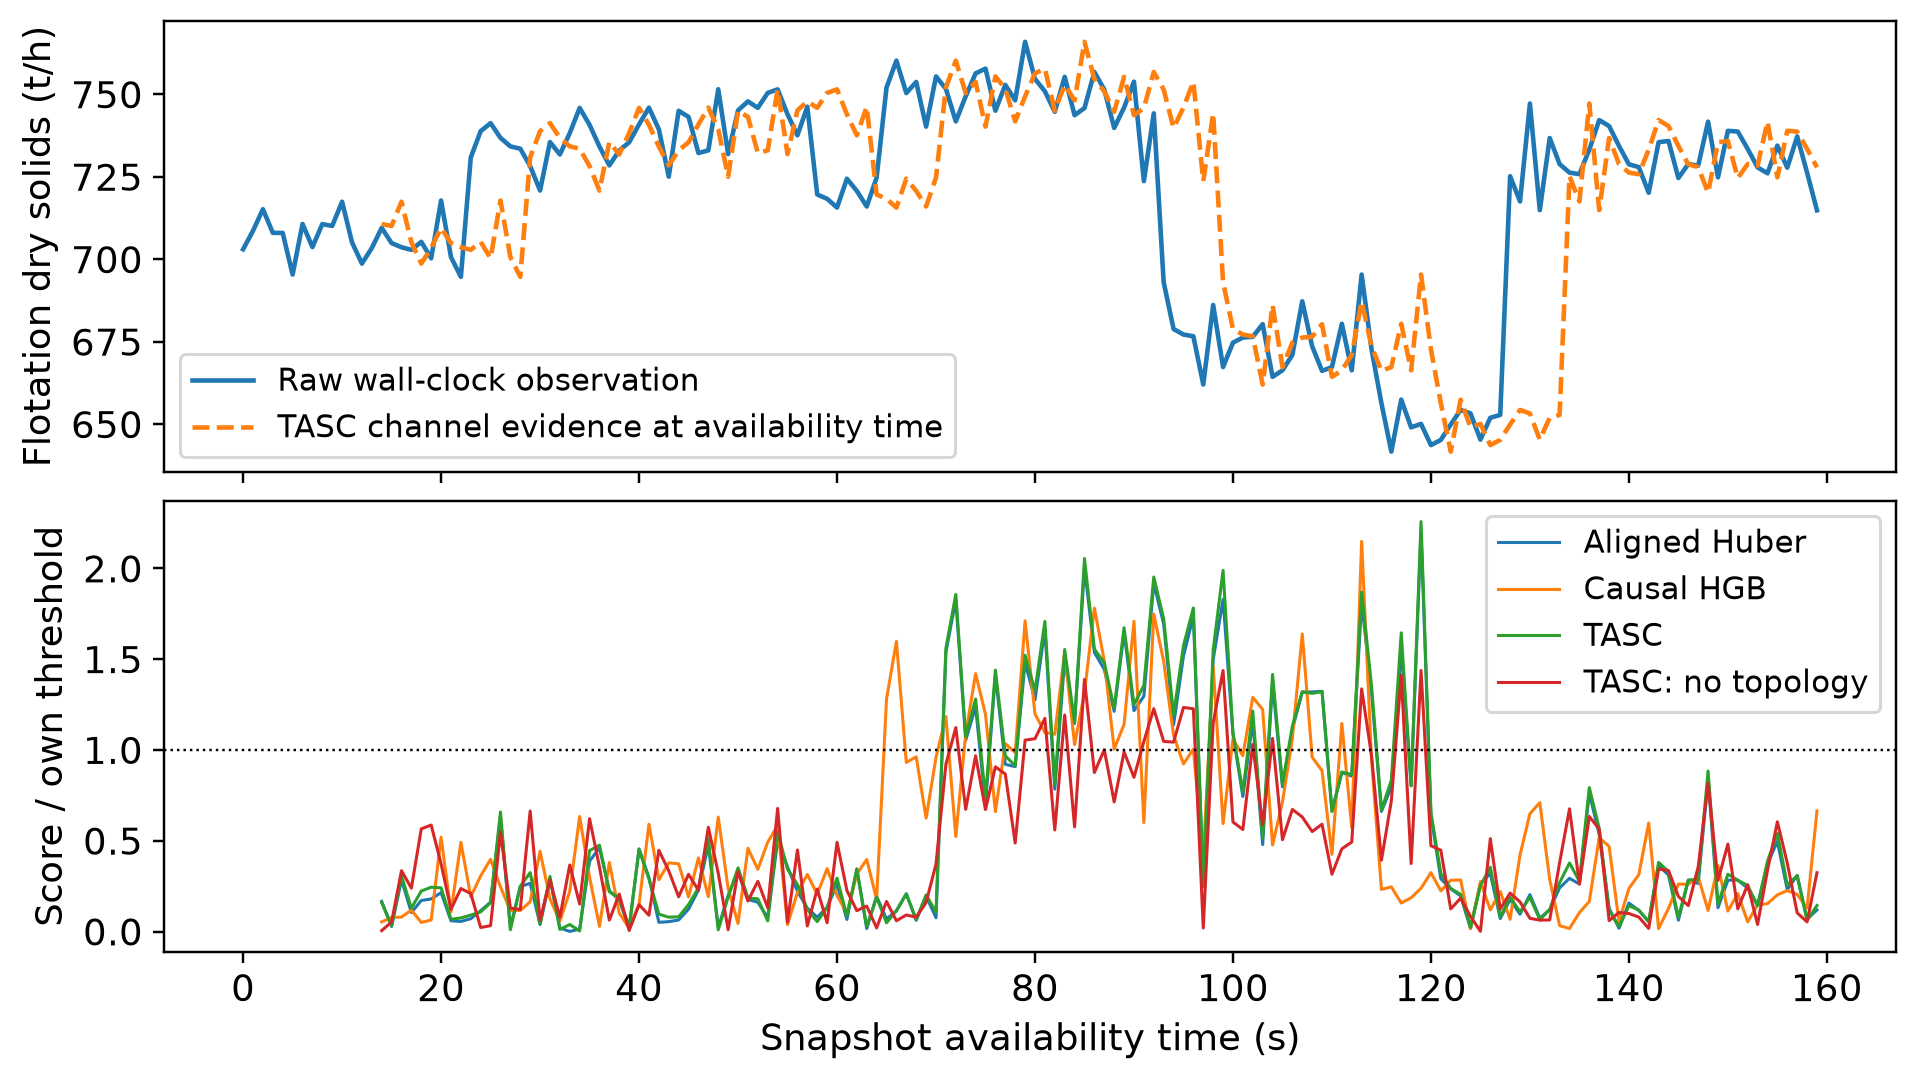
\includegraphics[width=.96\textwidth]{../shared/evidence-time.png}
\caption{Held-out flotation-feed bias. Earlier source evidence is displayed at its coherent snapshot availability time. Numerical scores use their own normal calibration; their common boundary of one does not make the algorithms' information sources equivalent.}
\end{figure}

\subsection{Imported geometry and resource behavior}
Every imported mapped node must identify a unique existing asset. World transforms include parent hierarchy transforms. Labels and incident stream endpoints are recomputed from the actual mapped objects; omitted assets lose their spatial overlays. Status-colored labels remain independent of imported materials, so an arbitrary mapped mesh need not contain a special reference marker.

The import boundary accepts glTF 2.0 within a 10\,MB file limit, 5000 nodes and two million accessor elements. Remote buffers/images and invalid transforms are refused. These constraints bound a local viewer, not general glTF security or engineering fidelity. Geometry exchange does not create new process equipment or certify an as-built coordinate system.

The scene renders on demand after state, camera, geometry, resize or theme changes. Continuous flow animation runs only during explicit replay. A paused model does not imply an active instrument connection, and a render-duration overlay is a measurement of the current browser rather than guaranteed plant latency. Keyboard asset selection and the process diagram remain available when spatial picking or WebGL is unsuitable.

\section{Actual CAOS engine evidence}
\subsection{Released packages and immutable artifacts}
Four exact released packages are executed: minehaulsim 0.12.1, bedblend 0.7.3, milldem 0.3.1 and oreblocks 0.6.6. Their public APIs respectively produce a constrained haulage reference, truck-dumped stockpile terrain, a short reduced-resolution charge transient and an authored porphyry pit solution. Configuration, seed, package identifier and result digest accompany the numeric outputs. The short charge calculation is qualitative context, not an industrial mill-power prediction.

Ten companion applications contribute exact public artifacts: ChancaDEM, OreFlow, PitForge, CutoffGrade, FragmentIQ, FrothSeg, TailWatch, RotorVitals, StockTwin and DispatchLab. Each is pinned by immutable source identifier, expected schema, bytes, SHA-256 and actual numeric path. A missing path, changed hash or non-finite metric refuses the import. Private or unpublished capabilities remain explicitly unavailable.

\begin{table}[htbp]\centering\small
\caption{Executed or verified external evidence. Release pins and declared software licenses identify the source; full immutable identifiers, hashes and extracted numeric paths are in the public source manifest. Original cases remain independent of the connected plant's synthetic observations.}
\begin{tabular}{p{.17\textwidth}p{.14\textwidth}p{.13\textwidth}p{.07\textwidth}p{.35\textwidth}}
\toprule Source & Pin & License & Asset & First extracted quantity\\\midrule
ChancaDEM & 0.11.000 & MIT & CR1 & Product P80 (mm)\\
OreFlow & 0.10.007 & MIT & FL1 & Copper recovery (\%)\\
PitForge & 0.14.000 & MIT & PIT & Oracle pit blocks (count)\\
CutoffGrade & 0.09.001 & MIT & PIT & Break-even copper grade (fraction)\\
FragmentIQ & 0.10.001 & MIT & ROM & Image-derived P80 (mm)\\
FrothSeg & 0.06.006 & MIT & FL1 & Bubble D32 (px)\\
TailWatch & 0.14.001 & MIT & MON & Reference false alarm rate (fraction)\\
RotorVitals & 0.48.001 & MIT & MOT & Shaft frequency (Hz)\\
StockTwin & 0.07.000 & MIT & ROM & Built stockpile volume (m3)\\
DispatchLab & 0.23.004 & MIT & TRK & Reference shift tonnes (t)\\
minehaulsim & 0.12.1 & Apache-2.0 & TRK & Shift output (t)\\
bedblend & 0.7.3 & MIT & ROM & Accepted loads (count)\\
milldem & 0.3.1 & MIT & SAG & Toe (deg)\\
oreblocks & 0.6.6 & MIT & PIT & Ultimate pit value (USD)\\
\bottomrule\end{tabular}

\end{table}

\subsection{Provenance is not calibration}
The selected examples are synthetic or analytic. The ten application sources use MIT; minehaulsim uses Apache-2.0, while bedblend, milldem and oreblocks use MIT. Each license remains attached to its source. No measured froth image, private vibration waveform or site geometry is reassigned to this plant. A verified file is evidence that a particular upstream calculation was consumed correctly. It is not evidence that the result applies to a different ore, machine, throughput or observation time.

The benchmark's uncertain prior is a fixed dry-solids relation anchored to one OreFlow operating reference. It is not a runtime merger of all fourteen external outputs. The visual integration can display each actual source while the numerical experiment remains intentionally narrower. This separation prevents the breadth of the interface from being mistaken for breadth of physical validation.

\section{Bounded downstream physical models}
\subsection{Settling transport and numerical resolution}
The separate one-dimensional column evolves solids volume fraction $\phi$ through a conservative finite-volume approximation,
\begin{equation}
 \frac{\partial\phi}{\partial t}+\frac{\partial}{\partial z}
 \left[v_b\phi+v_s\phi(1-\phi)^{4.65}\right]=S_f.
\end{equation}
A Rusanov flux and step bounded by a 0.4 CFL factor preserve the accounting of feed, outlets and stored solids. The implementation refuses fractions beyond its packing envelope rather than silently clipping an overloaded solution. Clarification/thickening literature provides the physical context~\cite{takacs}; the reference omits compression, flocculation kinetics and radial flow.

Default inputs are a 6\,m column, 40\,m$^2$ area, 20\,m$^3$/h feed at fraction 0.08, 8\,m$^3$/h underflow, settling coefficient 0.8\,m/h, initial solids fraction 0.06, mid-depth feed and a 2\,h transient. Conservation and resolution are distinct checks. Forty cells close solids accounting but substantially diffuse the outlet response. At 640 cells the endpoint fraction differs by 0.7562\% from a 2000-cell reference under these inputs. Other flows, durations or constitutive parameters require their own refinement.

\begin{figure}[htbp]\centering
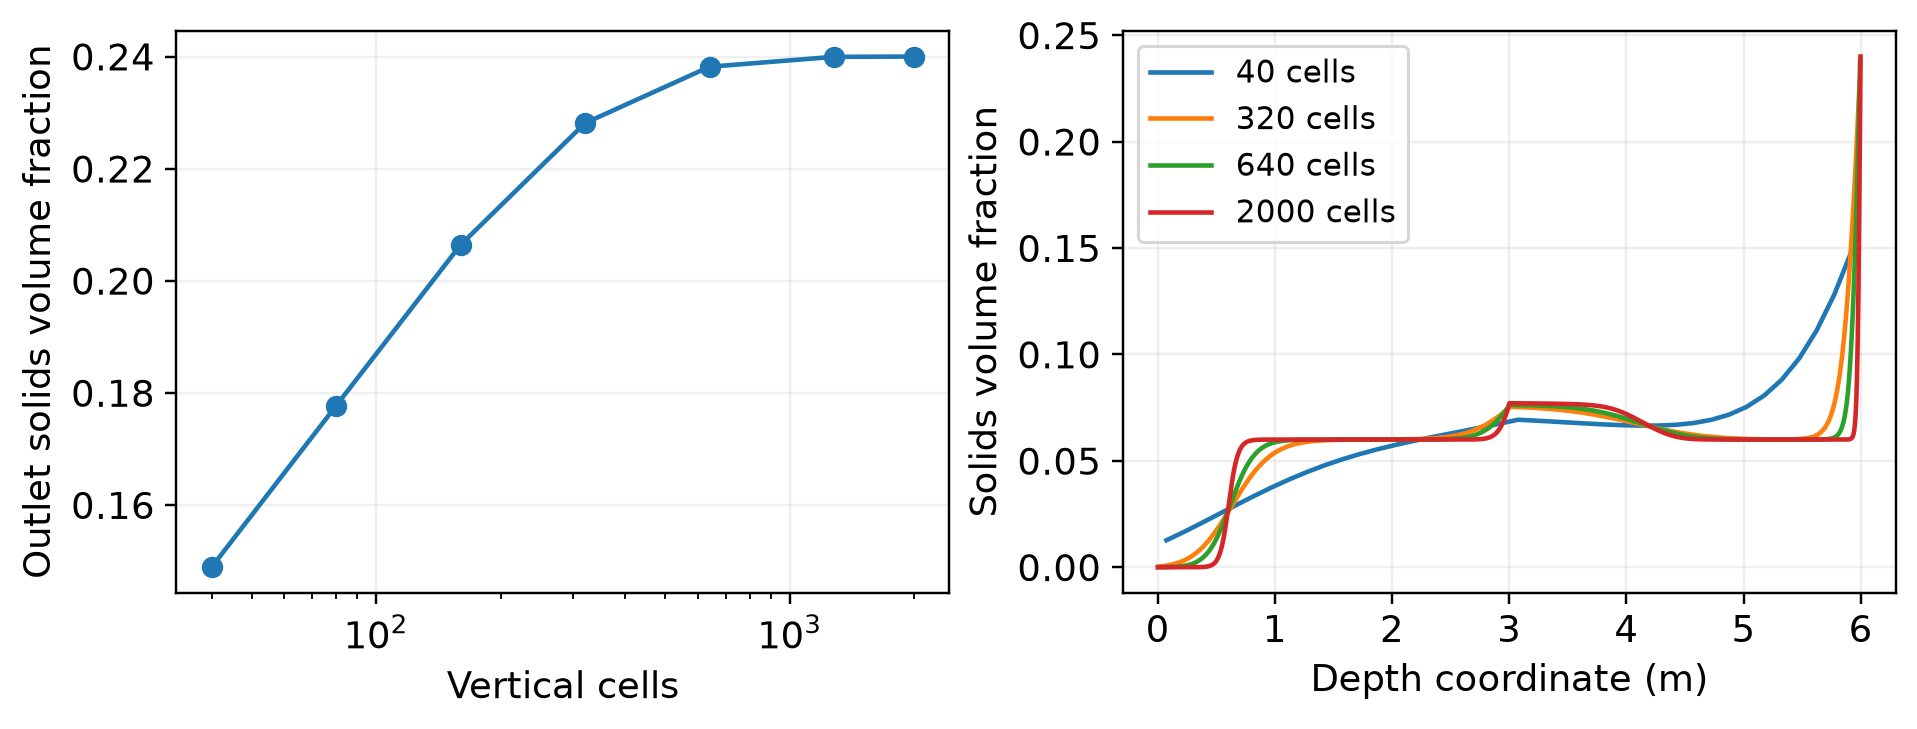
\includegraphics[width=.98\textwidth]{../shared/grid-study.png}
\caption{Actual grid-refinement calculations. Exact feed/outlet/inventory accounting does not guarantee an adequately resolved concentration profile. The reference is independently parameterized from the displayed plant thickener.}
\end{figure}

The 640-cell transient releases approximately 0.290800\,m$^3$ of initial solids inventory. Its integrated balance is
\begin{equation}
 V_{in}-V_{out}=M_{final}-M_{initial}.
\end{equation}
All four terms are integrated solids volumes in cubic metres: incoming and outgoing solids, and final and initial stored solids. Ignoring storage would manufacture measurement corrections even when numerical accounting is exact. This example illustrates the missing term; the sixteen-channel detection experiment does not infer dynamic vessel inventories.

\subsection{Leach conversion and acid limit}
The particle conversion $X$ follows a combined reaction/diffusion shrinking-core reference,
\begin{equation}
 t=\tau_r[1-(1-X)^{1/3}]
 +\tau_d[1-3(1-X)^{2/3}+2(1-X)],
\end{equation}
with authored reaction and diffusion times of 2 and 4\,h. The CSTR conversion averages the monotone particle response over an exponential age distribution with mean residence $\tau$:
\begin{equation}
 \overline X(\tau)=\int_0^\infty X(t)\frac{e^{-t/\tau}}{\tau}\,dt.
\end{equation}
This ideal residence calculation is not a reactive heap transport model. The reaction-controlled limit has an independent closed form. Kinetics and mineral compatibility need independent calibration; cited heap/bioleach modeling includes mechanisms outside this reference~\cite{leahy}.

For feed copper rate $\dot m_f$, available acid $\dot m_A$ and coefficient $a=1.543$\,kg acid/kg Cu,
\begin{equation}
 \dot m_{dissolved}=\min(\dot m_f\overline X,\dot m_A/a),\qquad
 \dot m_{residue}=\dot m_f-\dot m_{dissolved}.
\end{equation}
The default route dissolves approximately 411.1237\,kg/h. Acid and copper closure are checked independently. The coefficient and conversion parameters describe the authored reference rather than arbitrary ore chemistry.

\subsection{Ideal solvent extraction and electrowinning}
Two ideal crosscurrent contacts use fresh organic at each stage. With aqueous flow $Q_a$, organic flow per stage $Q_o$, distribution ratio $K$ and initial aqueous concentration $C_0$,
\begin{equation}
 C_n=C_0\left(\frac{Q_a}{Q_a+KQ_o}\right)^n.
\end{equation}
Default values are $Q_a=150$\,m$^3$/h, $Q_o=120$\,m$^3$/h per stage, $K=2$ and $n=2$. Total fresh organic is 240\,m$^3$/h. Approximately 350.3066\,kg/h Cu transfers; the remaining aqueous copper closes the balance. This is not an industrial countercurrent mixer-settler simulation.

Electrowinning uses two-electron charge accounting~\cite{ew}:
\begin{equation}
 \dot m_{cathode}=\min\left(\dot m_{available},
 \frac{3600\eta I M_{Cu}}{2F}\right),\quad
 P=IV/1000,
\end{equation}
where $M_{Cu}=0.063546$\,kg/mol and $F=96485.33212$\,C/mol. At $I=400$\,kA, efficiency 0.92 and 2.1\,V, solution copper limits cathode production to approximately 350.3066\,kg/h at 840\,kW. Specific energy is approximately 2.3979\,kWh/kg. Increasing current after the solution limit raises power without raising this calculated output. The browser computes the same bounded route and is compared with Python at common inputs.

\section{Numerical state and discrepancy methods}
\subsection{Engineering thresholds and weighted reconciliation}
For positive authored nominal $\mu_i$, the independent threshold score is $|y_i-\mu_i|/(0.20\mu_i)$. Values above one indicate a discrepancy. These nominal margins are reference choices, not approved site operating limits.

Weighted reconciliation minimizes
\begin{equation}
 \frac12(y-x)^T\Sigma^{-1}(y-x)\quad\hbox{subject to }Ax=b,
\end{equation}
with diagonal $\Sigma_{ii}=\max(0.01\mu_i,0.1)^2$. The reusable solver supports redundant equations through a rank-aware least-squares projection and rejects inconsistent constraints. With no constraints it returns the observations. The batch experiment uses eleven independent homogeneous factors and complete finite frames.

\subsection{Huber projection and fixed calibration}
Huber loss is quadratic for $|r|\le1.5$ and linear beyond that transition. Iterative reweighting uses
\begin{equation}
 w_i^{(k)}=\min\left(1,\frac{1.5}{\max(|(x_i^{(k)}-y_i)/\sigma_i|,10^{-12})}\right).
\end{equation}
The reusable single-frame routine allows 25 iterations; the vectorized experiment allows 30 with maximum-change tolerance $10^{-7}$. Normal state-calibration seeds 300--307 fix the higher 99.5th percentile of each score, bounded below by 0.1. Displayed scores divide by these fixed boundaries. Neither iteration convergence nor a small equality residual establishes fault identifiability.

\subsection{Causal histogram prediction}
The fitted model predicts sixteen next-step channels from four earlier multichannel vectors, giving 64 lag features. Normal training uses eight 200-sample sequences from seeds 100--107: 1568 target rows after lag construction. Forecast calibration uses seeds 200--203 and 784 rows. Each channel regressor uses 70 boosting iterations, at most 12 leaves, 64 bins, L2 regularization 1 and random seed 41. Training-target standard deviations scale inputs and targets.

Absolute prediction errors on disjoint normal calibration define higher 99.5th-percentile channel thresholds, bounded below by $10^{-8}$. Test labels never set these parameters. Rejected source values are masked before lag preparation. Last accepted values are carried only inside model input, with nominal initialization before the first accepted sample. Display and scoring retain the rejected target state; missing information is not physically restored.

\subsection{Regularized linear causal prediction}
A second fitted family uses native multioutput ridge regression on the same four earlier multichannel vectors. With $\tilde X\in\mathbb R^{1568\times64}$, $\tilde Y\in\mathbb R^{1568\times16}$, coefficient matrix $W\in\mathbb R^{16\times64}$ and intercept $b\in\mathbb R^{16}$,
\begin{equation}
 (\widehat W,\widehat b)=\arg\min_{W,b}\|\tilde Y-\tilde XW^T-\mathbf1b^T\|_F^2+\alpha\|W\|_F^2,\qquad\alpha=1.
\end{equation}
The squared residual sum is unaveraged; the intercept is unpenalized. Native multiple targets share the input design without estimating a coupled output-error covariance. Ridge is a regularized linear causal predictor, not an advanced nonlinear model merely because its implementation is maintained~\cite{ridge}.

The training-target standard deviation scales both targets and the corresponding channels repeated across four lags. This division does not itself subtract a mean; the fitted intercept accounts for the offset. Predictions return to each channel's original units before absolute-error calibration. Training seeds 100--107, normal calibration seeds 200--203, higher 99.5th-percentile thresholds and the common fourteen-sample numerical horizon match the histogram protocol. Rejected finite values are removed before carry-forward; an inconsistent mask admitting a non-finite target is refused.

The linear penalty, SVD solver and intercept setting were fixed before viewing the added aggregate. The test seeds were already known from the published controlled study. This is a post-publication extension rather than prospectively untouched model selection. The additional artifact reuses the original 768 histogram rows and adds 768 ridge evaluations; it does not create 1536 independent new trials. The original eight-method counts, paired analysis and twelve trace byte sequences are preserved.

\subsection{Transport-aware fusion and ablations}
TASC combines aligned observations with compatible uncertain pseudo-observations under the same conservation factors:
\begin{equation}
 \min_{Ax=0}\sum_i\rho_{1.5}\left(\frac{x_i-y_i^{aligned}}{\sigma_i}\right)
 +\sum_{i\in E}\rho_{1.5}\left(\frac{x_i-m_i}{\tau_i}\right).
\end{equation}
For the twelve dry-solids channels, $m_i=y_0^{aligned}\mu_i/\mu_0$ and $\tau_i=\max(0.04\mu_i,0.4)$. Four water channels have no prior from this dry-solids relation. Clean truth and injected fault labels never enter the prior.

Removing the prior reproduces aligned Huber. Removing timing uses simultaneous readings. Removing topology removes equality factors while retaining the compatible prior. Those variants test the mechanisms under a fixed authored process. They do not establish that conservation is useless generally. The current batch withholds a complete constrained frame when any required observation is invalid; the separate single-row implementation has an explicitly narrower missing-input admission rule and can expose algebraic factor membership. Neither is a validated industrial diagnosis system.

\section{Controlled experiment}
\subsection{Families, splits and dependence}
The experiment spans twelve families: healthy load transition, feed bias, cyclone drift, frozen source, incompatible unit, incorrect binding, missing observation, out-of-order sequence, concentrate imbalance, changed recovery relation, water discrepancy and unmodeled transport delay. Known quality masks emulate an ingestion decision; they are not a learned source-fault detector.

Sixteen held-out seeds, 1000--1015, and four severity slots, 0.5, 1, 2 and 4, produce 768 protocol scenarios and 6144 method/scenario cells. Noise scale is fixed at one. Magnitude-bearing disturbances change with severity. Healthy/delay controls and known quality-rejection families repeat across those slots; they are not independent new experiments. Complete seed blocks retain this dependence in uncertainty calculations.

Each trace has 160 one-second samples and sixteen channels. The common numerical horizon has 146 samples after fourteen history samples. Aligned methods use causally aligned truth. The changed-recovery family updates current physical truth and is balanced at simultaneous raw time; unequal channel alignment can introduce transient factor residuals at its boundaries. It therefore tests both a changed fixed-prior relation and alignment effects, rather than isolating prior compatibility. Its affected coordinates are process-change labels, not proof of an instrument fault. The delay family changes healthy process timing and has no sensor-fault label. Its alerts count as false for the defined fault-detection task, even though a transport change may be operationally interesting.

\subsection{Metrics and refusal support}
Numerical precision, recall and false-positive rate are
\begin{equation}
 P=\frac{TP}{TP+FP},\qquad R=\frac{TP}{TP+FN},\qquad
 FPR=\frac{FP}{FP+TN}.
\end{equation}
Undefined denominators remain absent. No point adjustment expands one alarm over an entire event. A scored point belongs to exactly one confusion cell, and scored plus unscorable equals the common horizon. Complete-frame projection loses more score support than per-target threshold/prediction methods when one source is rejected.

Event aggregation is separate from pointwise scoring. Detection latency is finite only if a same-channel true positive occurs during the affected support. A late false alert after a missed event cannot create a successful detection. Latency is the time of the first localized true positive minus the first comparable aligned-label availability. It excludes alignment waiting time from the original raw fault onset and is not a field communication-delay measurement.

Paired percentile intervals use 5000 resamples of the sixteen complete test-seed blocks with random seed 414. Family, severity, channel and time dependence remain together. A source-valid analysis also removes all five quality-rejection families, leaving 448 common-support scenario slots. The intervals describe this synthetic process and its weighting, without estimating industrial population uncertainty.

\section{Measured comparisons}
\subsection{Detection, false alerts and coverage}
Table~\ref{tab:results} gives pooled pointwise results. The engineering threshold has no false alerts in this matrix but recall only 0.3065. That observation does not make its field false-positive probability zero. Simultaneous WLS has recall 0.1481; aligned Huber reaches 0.3362. The causal predictor has recall 0.8399 and false-positive rate approximately 0.01591 after rejected finite values are excluded from its feature history.

\begin{table}[htbp]\centering\scriptsize
\caption{Full controlled experiment. Ratios use valid finite scores. Coverage is the fraction of the common numerical horizon that receives a score.}\label{tab:results}
\begin{tabular}{lrrrrrrr}\toprule
Method & TP & FP & FN & Precision & Recall & FPR & Coverage \\
\midrule
Engineering threshold & 9808 & 0 & 22192 & 1.0000 & 0.3065 & 0.00000 & 0.9911 \\
WLS & 4739 & 14475 & 27261 & 0.2466 & 0.1481 & 0.00961 & 0.8573 \\
Aligned Huber & 10759 & 13501 & 21241 & 0.4435 & 0.3362 & 0.00896 & 0.8573 \\
Causal HGB & 26878 & 27780 & 5122 & 0.4917 & 0.8399 & 0.01591 & 0.9911 \\
TASC & 10941 & 13376 & 21059 & 0.4499 & 0.3419 & 0.00888 & 0.8573 \\
TASC: no timing & 7512 & 10012 & 24488 & 0.4287 & 0.2347 & 0.00665 & 0.8573 \\
TASC: no prior & 10759 & 13501 & 21241 & 0.4435 & 0.3362 & 0.00896 & 0.8573 \\
TASC: no topology & 16611 & 8720 & 15389 & 0.6558 & 0.5191 & 0.00579 & 0.8573 \\
\bottomrule\end{tabular}

\end{table}

TASC reaches recall 0.3419, precision 0.4499 and false-positive rate approximately 0.00888. Removing topology improves recall to 0.5191 and precision to 0.6558. Removing the prior reproduces aligned Huber. Removing timing reduces both recall and false alerts, a tradeoff rather than evidence of an unqualified improvement. The source-valid subset preserves the unfavorable recall ordering.

\begin{figure}[htbp]\centering
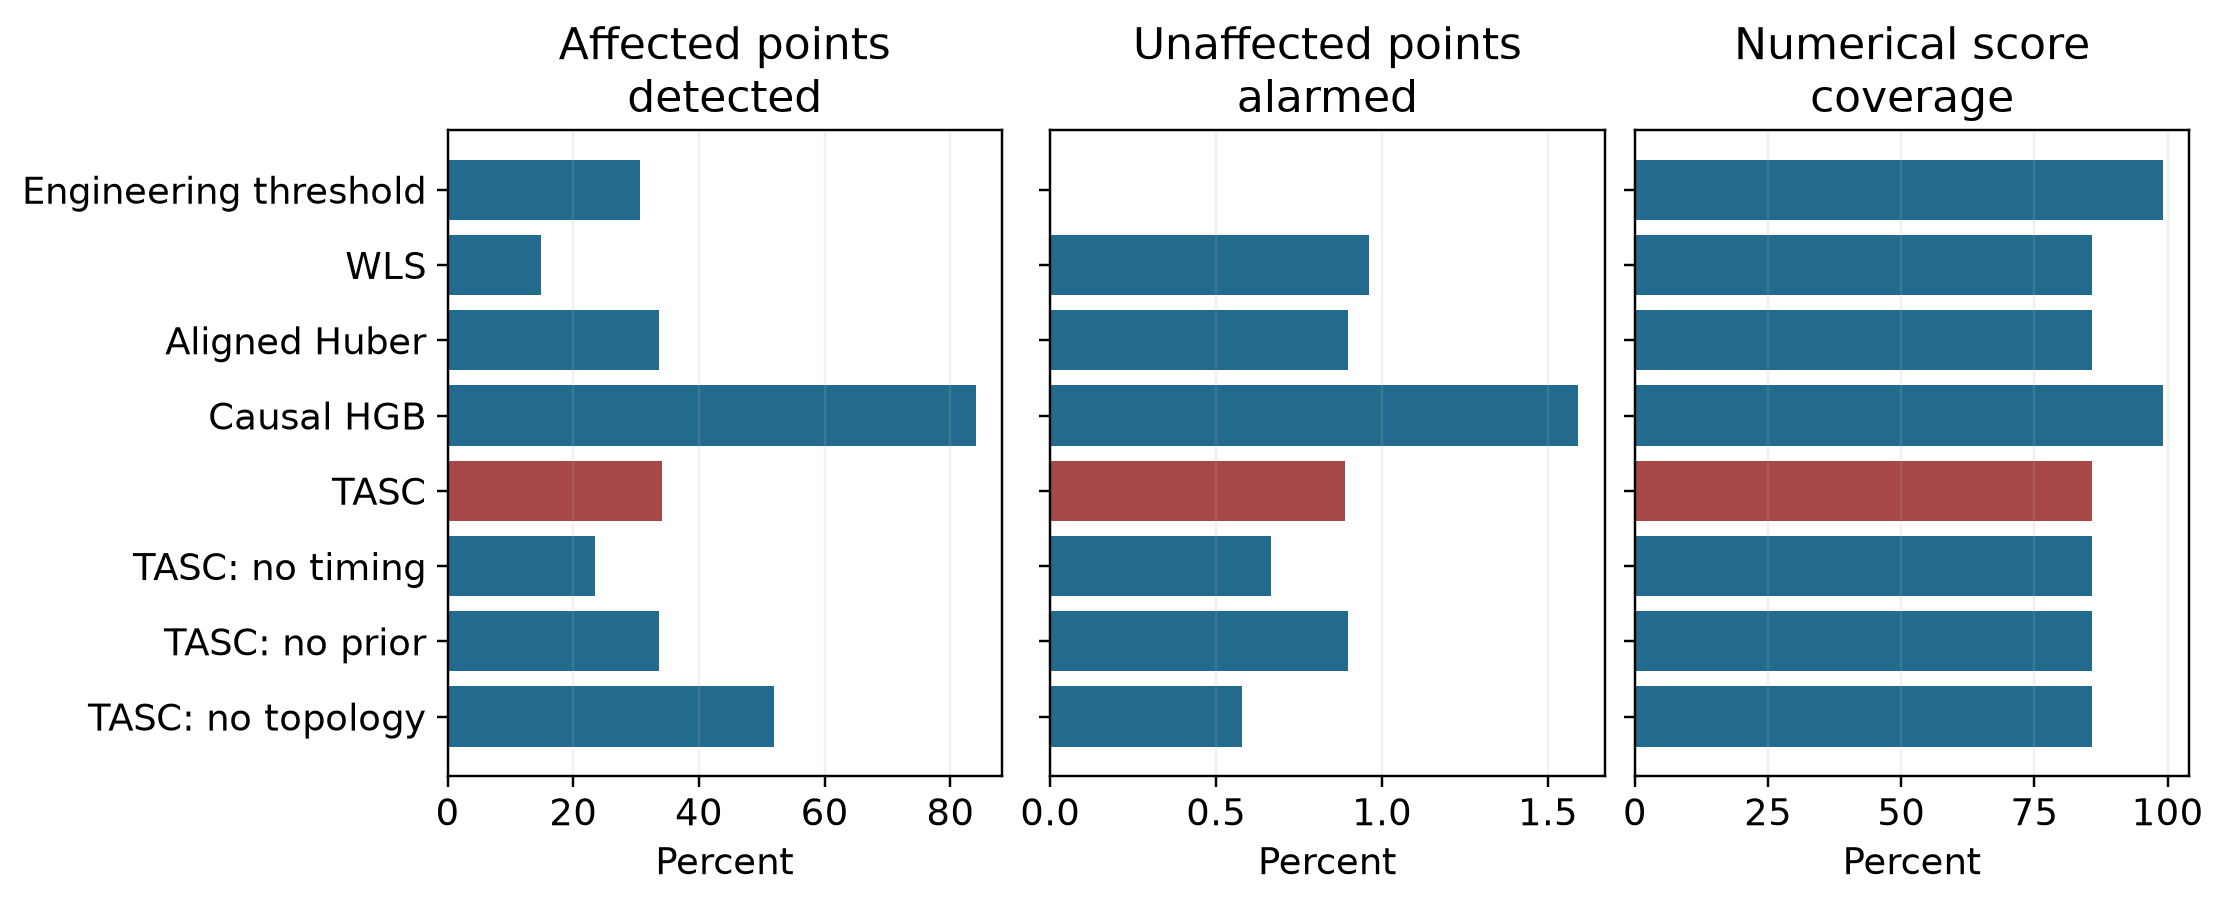
\includegraphics[width=\textwidth]{../shared/comparison.png}
\caption{All eight alternatives, including every ablation. Detection, false-alert rate and score coverage have different denominators; lower alert rate with larger refusal support is not a free accuracy gain.}
\end{figure}

Complete-frame methods have 256000 unscorable entries, compared with 16000 for the independent threshold and forecast. Source-invalid coordinates are excluded from numerical scoring; constrained methods additionally withhold other coordinates of those incomplete frames. This difference affects false-positive denominators and must accompany any pooled comparison.

\subsection{Paired uncertainty and severity}
TASC minus aligned-Huber recall is 0.0056875, with paired 95\% interval $[0.0043750,0.0070938]$. Its recall difference from the predictor is $-0.4980312$, interval $[-0.5293133,-0.4610281]$. The difference from no-topology is $-0.1771875$, interval $[-0.1792188,-0.1752812]$. The small positive gain over aligned Huber coexists with much larger losses to the other comparisons.

\begin{figure}[htbp]\centering
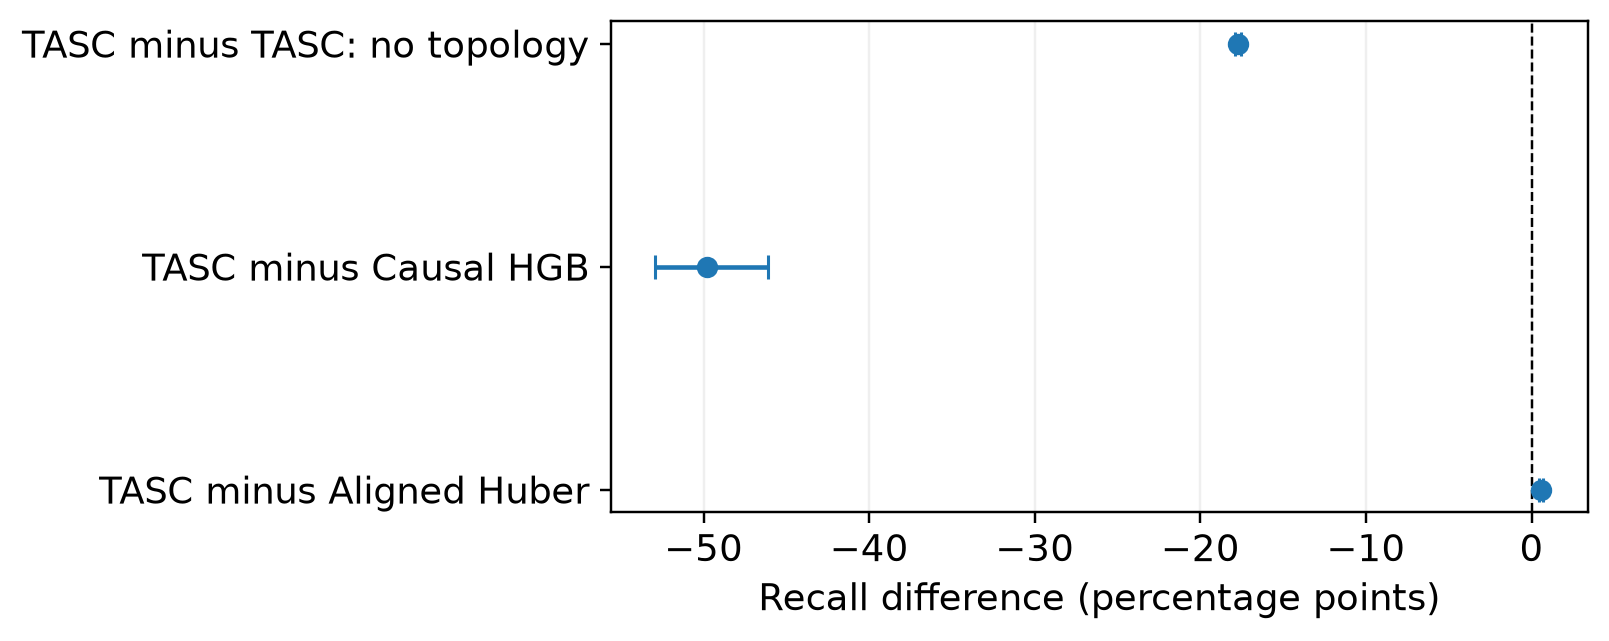
\includegraphics[width=.95\textwidth]{../shared/paired.png}
\caption{Paired recall differences using complete seed blocks. The narrow negative interval against no-topology applies to this authored process and fixed prior, not to every conservation-based estimator.}
\end{figure}

\begin{figure}[htbp]\centering
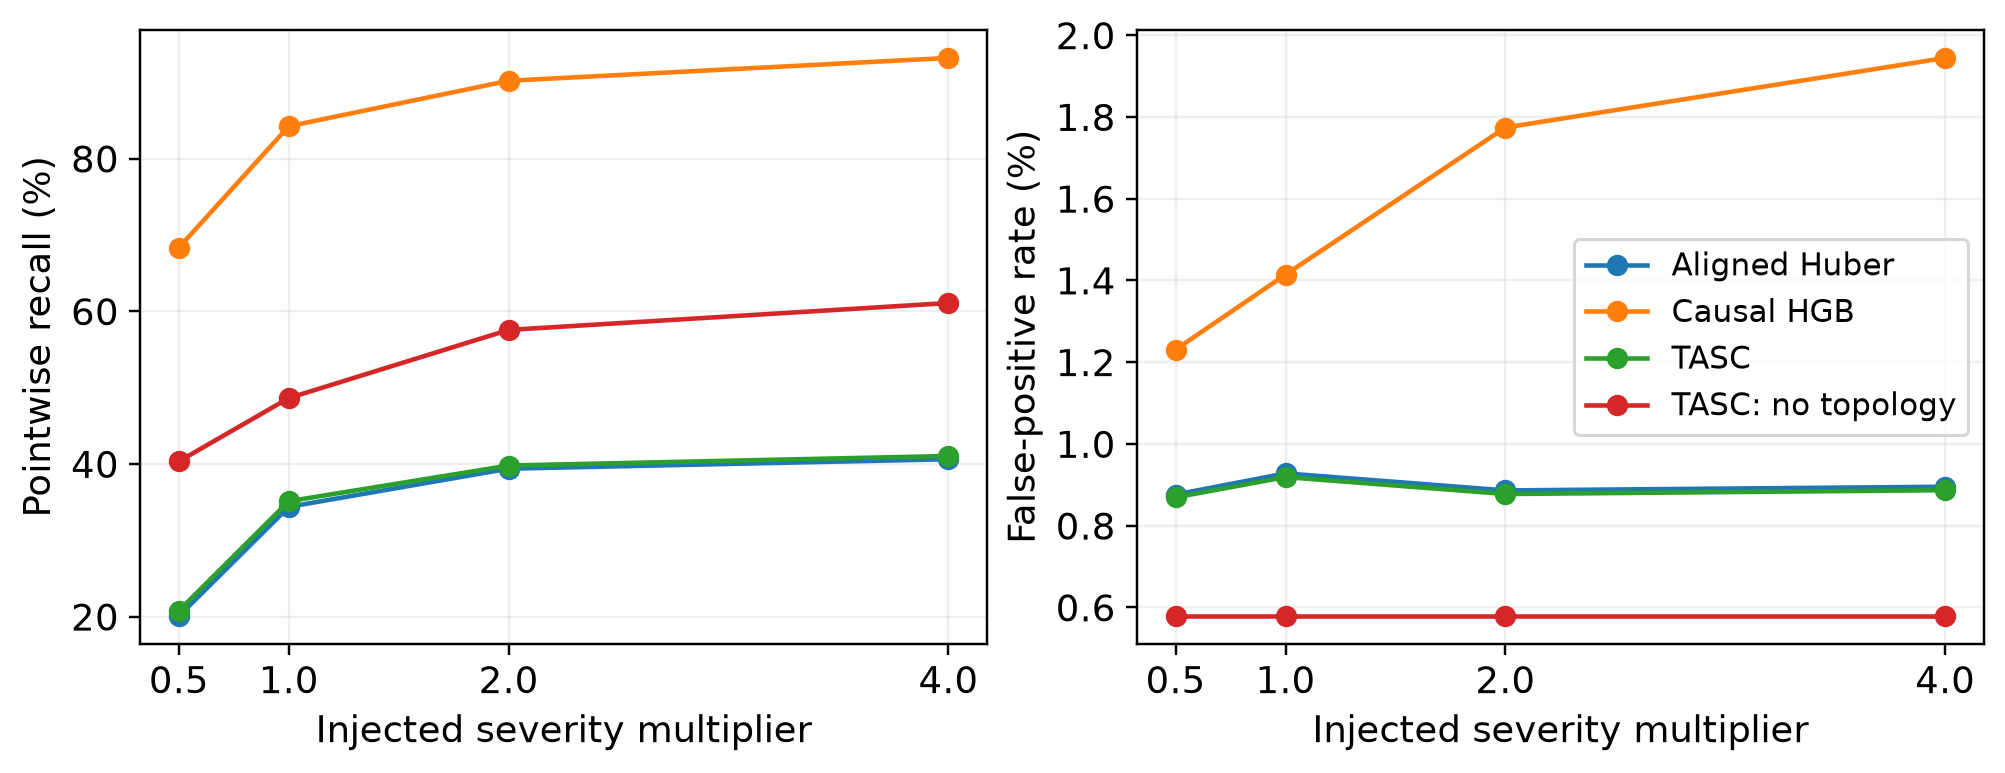
\includegraphics[width=.98\textwidth]{../shared/severity.png}
\caption{Measured severity response at fixed noise scale. Repeated controls and quality scenarios retain the same protocol weight at each slot. Curves summarize the controlled matrix rather than a distribution of industrial failure magnitudes.}
\end{figure}

\subsection{Paired extension with a second fitted family}
Ridge has 29454 true positives, 51003 false positives and 2546 false negatives. Its recall is 0.9204375, precision 0.3660837 and false-positive rate 0.0292105, compared with 0.8399375, 0.4917487 and 0.0159102 for the histogram model. Both score 1778048 points and leave 16000 unavailable. Higher recall therefore accompanies more false alerts and lower precision; the linear family is not uniformly better.

The ridge-minus-histogram recall difference is 0.0805. A 5000-resample, seed-414 bootstrap over the same sixteen complete seed blocks gives the 95\% interval $[0.0482797,0.1189695]$. Family, severity, channel and time dependence remain inside each block. Reused test slots and supplied admission masks limit this interpretation to the authored design.

\begin{figure}[htbp]\centering
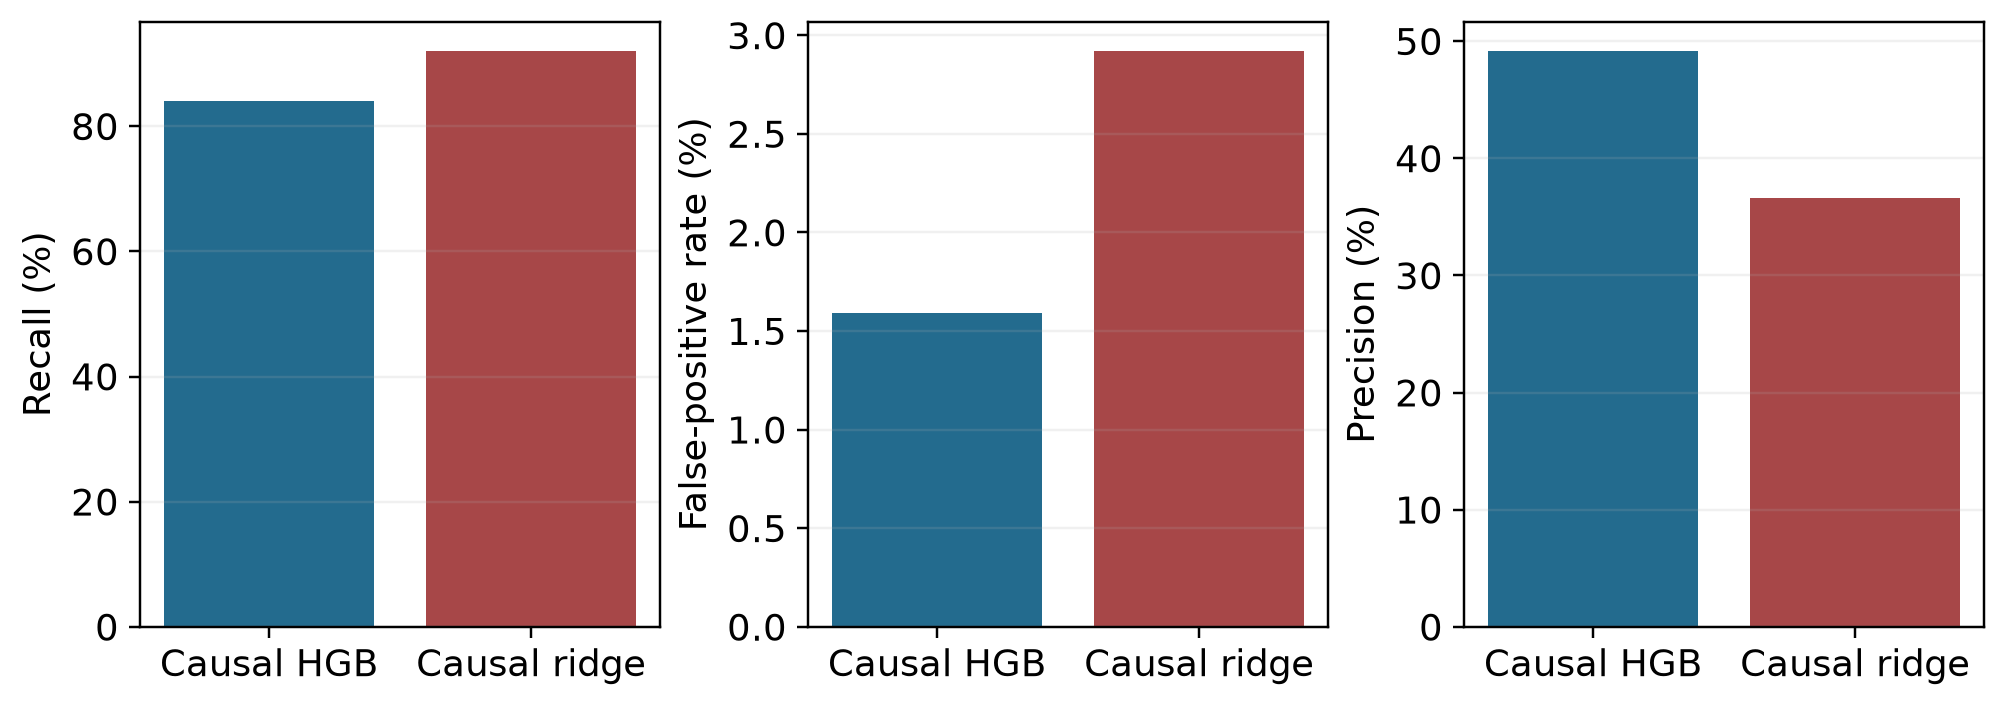
\includegraphics[width=.98\textwidth]{../shared/ridge-comparison.png}
\caption{The additional fitted linear family gains recall at a higher false-alert rate. These are paired records on the already-known synthetic protocol, including 768 reused histogram rows. No universal advantage is inferred.}
\end{figure}

Independent augmented least squares reproduces ridge coefficients to approximately $3.1\times10^{-14}$, the intercept to $2.2\times10^{-14}$ and original-unit predictions to $4.0\times10^{-12}$. Separate recomputation from the actual checkpoint reconciles all 768 ridge counts and event latencies, its higher-quantile calibration and the paired interval. Missing model manifests, wrong checkpoint identities and missing or duplicate protocol cells fail validation.

\subsection{Why closure can hurt localization}
A balance factor observes a syndrome, not an instrument identity. In a three-channel flotation balance, an extra 10\,t/h at feed and a missing 10\,t/h at tailings produce the same scalar residual. One equation leaves two unconstrained physical directions. A unique weighted optimum comes from uncertainty assumptions; it does not eliminate that ambiguity.

Projection can spread one contaminated observation among correlated channels. A graph-local correction may therefore appear persuasive while mislocalizing the underlying disturbance. The negative no-topology comparison indicates that the particular equality/prior combination is not justified as a generally better detector on this process. A different site, storage model or uncertainty structure requires a new held-out experiment, not retrospective threshold adjustment.

\section{Independent numerical and software verification}
Weighted solutions were compared with independent constrained/KKT calculations. Forty-eight robust systems were independently optimized in constraint null spaces; maximum objective differences were at numerical precision. Aggregate counts were recomputed over all 6144 cells. Scored-point counts match numerical denominators, and wholly missed events have no finite latency.

All four released package configurations were re-executed and their result digests reproduced. The ten exact public artifacts matched expected bytes, SHA-256, schema and extracted metrics. This substantiates actual source consumption separately from any claim about the synthetic plant's applicability.

Channel snapshot checks resolved 245760 method/channel/time values to their exact evidence indices. Imported hierarchy transforms moved labels and stream endpoints together; omitted mappings removed their spatial overlays. Wrong tag/asset/unit tuples, decreasing sequences, timezone-naive times, conversion overflow and invalid stream dimensions were refused. Real local OPC UA server/client tests and separate browser transport tests examine different parts of the source boundary.

Four progressive bilingual lesson pairs, eight EN/ES notebook files, import the maintained methods. They execute weighted correction sensitivity, healthy transport alignment, changing solids inventory, identical-input Huber/HGB comparison, missingness, ambiguity and full paired analysis. Every lesson has numerical answers, figures and explicit limitations. Fresh copied executions reproduce their accepted output bytes. Successful execution alone would not establish physical interpretation; the inventory sign and null-ratio meanings are checked as part of the scientific explanation.

\section{Limitations and applicability}
The sixteen-channel generator is a short authored process anchored to one reference. It omits many chemical changes, maintenance states, nonlinear dynamics, correlated measurement errors and industrial modes. Known quality masks emulate input rejection. Delay and uncertainty metadata are assumed, not estimated from field instruments. The current constrained batch does not infer dynamic inventory or general missing-coordinate observability.

The fourteen external sources retain independent cases. Their breadth cannot be interpreted as fourteen calibrated models of one operating plant. The fixed dry-solids prior covers no water chemistry and is not a live engine ensemble. Algebraic factor membership and an interpretable diagram are not automatic root-cause diagnosis. No site historian, surveyed geometry, production authorization or operator acceptance establishes external validity.

The settling column's convergence result applies only to its default input. Its geometry and throughput do not size the displayed thickener. Ideal crosscurrent SX, shrinking-core kinetics and Faraday accounting exclude industrial countercurrent transport, mineral-general chemistry and electrochemical side effects beyond the stated efficiency. No tailings stability or safe operating assurance follows from an equipment view.

A visual integration may still be useful for inspecting relationships, provenance and missing data when these boundaries are explicit. Evaluating operational benefit requires measured site use, independently calibrated mappings/time support and outcomes that remain favorable under held-out operating regimes.

\section{Reproduction and availability}
The public repository supplies source, source lock, compact observations, metadata for both fitted families, comparison counts, paired analysis, notebook outputs and figure code. External roots hold raw caches, the trusted joblib checkpoint and temporary computations. Each checkpoint digest is in its model manifest; an unknown serialized model must not be loaded merely because it has a filename resembling the expected one.

The numerical environment uses Python 3.12.10, NumPy 2.2.6, SciPy 1.18.1 and scikit-learn 1.9.1 with numerical thread counts bounded to one. The full comparison using the fitted checkpoint took approximately 80.3\,s on the recorded workstation. Transfer size, render duration and numerical runtime describe that configuration, not arbitrary larger facilities.

The source and model commands are \texttt{run.py sources}, \texttt{run.py all --benchmark}, and the separately available infer/evaluate/export stages. Training, both calibration groups and test seeds are separated before inference. Scientific source, compact data and computational material are available at \url{https://github.com/fsantibanezleal/CAOS_OreBridge}. The software release supplies the external checkpoint separately from the scientific articles.

\section{Conclusions}
A connected plant view can preserve equipment identity, dimensional meaning, source quality and causal evidence time while consuming actual independent process-engine outputs. The implementation provides synchronized geometry, directed diagrams, observations and provenance, together with a bounded read-only source path.

The controlled models also expose a substantive limitation: robust conservation fusion does not automatically improve discrepancy localization. TASC's small recall gain over aligned Huber is outweighed by losses to causal prediction and its no-topology ablation in this experiment. Retaining coverage and those comparisons is necessary before interpreting an equipment color as evidence about a physical process.

\begin{thebibliography}{99}
\small\raggedright
\bibitem{sadeghi} Sadeghi, Hodouin and Bazin (2018). Mineral processing plant data reconciliation including mineral mass balance constraints. \emph{Minerals Engineering}. \url{https://doi.org/10.1016/j.mineng.2018.04.023}.
\bibitem{huber} Huber, P. J. (1964). Robust Estimation of a Location Parameter. \emph{Annals of Mathematical Statistics}, 35, 73--101. \url{https://doi.org/10.1214/aoms/1177703732}.
\bibitem{hgb} scikit-learn. HistGradientBoostingRegressor, maintained documentation, 1.9.1. \url{https://scikit-learn.org/stable/modules/generated/sklearn.ensemble.HistGradientBoostingRegressor.html}.
\bibitem{gdn} Deng, A. and Hooi, B. (2021). Graph Neural Network-Based Anomaly Detection in Multivariate Time Series. \emph{AAAI}. \url{https://arxiv.org/abs/2106.06947}.
\bibitem{gstpro} Zheng, Y. et al. (2024). Graph Spatiotemporal Process for Multivariate Time Series Anomaly Detection with Missing Values. \url{https://arxiv.org/abs/2401.05800}.
\bibitem{datavalue} OPC Foundation. OPC Unified Architecture, Part 4: Services, section 7.11, DataValue. \url{https://reference.opcfoundation.org/specs/OPC-10000-4/7.11}.
\bibitem{opc-security} OPC Foundation. OPC Unified Architecture, Part 2: Security Model. \url{https://reference.opcfoundation.org/specs/OPC-10000-2/full}.
\bibitem{mining} OPC Foundation. OPC UA for Mining, General, 1.01.0. \url{https://reference.opcfoundation.org/specs/OPC-40560/full}.
\bibitem{gltf} Khronos Group. glTF 2.0 specification. \url{https://registry.khronos.org/glTF/specs/2.0/glTF-2.0.html}.
\bibitem{dexpi} DEXPI. Specifications for process and plant engineering exchange. \url{https://dexpi.org/specifications/}.
\bibitem{azure} Microsoft. Use 3D Scenes Studio in Azure Digital Twins. \url{https://learn.microsoft.com/en-us/azure/digital-twins/how-to-use-3d-scenes-studio}.
\bibitem{aws} Amazon Web Services. AWS IoT TwinMaker knowledge graph and scenes. \url{https://docs.aws.amazon.com/iot-twinmaker/latest/guide/tm-knowledge-graph-scene.html}.
\bibitem{takacs} Takács, Patry and Nolasco (1991). A dynamic model of the clarification-thickening process. \emph{Water Research}, 25, 1263--1271. \url{https://doi.org/10.1016/0043-1354(91)90066-Y}.
\bibitem{leahy} Leahy, Davidson and Schwarz (2005). A model for heap bioleaching of chalcocite with heat balance: Bacterial temperature dependence. \emph{Minerals Engineering}. \url{https://doi.org/10.1016/j.mineng.2005.07.003}.
\bibitem{ew} Dehkhoda, A. M. and Wassink, B. Electrowinning fundamentals. \emph{Aqueous Pathways}. BCcampus. \url{https://pressbooks.bccampus.ca/hydrometallurgy/chapter/electrowinning-fundamentals/}.
\bibitem{cochilco-energy} Cochilco. Proyección del consumo de energía eléctrica en la minería del cobre, período 2025--2034. \url{https://www.cochilco.cl/web/informe-proyeccion-del-consumo-de-energia-electrica-en-la-mineria-del-cobre-periodo-2025-2034-2/}.
\bibitem{cochilco-water} Cochilco. Proyección de la demanda de agua en la minería del cobre en Chile, período 2025--2034. \url{https://www.cochilco.cl/web/https-www-cochilco-cl-web-download-1014-2026-15581-informe-proyeccion-de-la-demanda-de-agua-en-la-mineria-del-cobre-en-chile-periodo-2025-2034-pdf/}.
\end{thebibliography}

\end{document}
